%!TEX root = mieic-en.tex

\chapter{Implementation}\label{chap:chap4}
\section*{}

\textit{
Este capítulo pode ser dedicado à apresentação de detalhes de nível
mais baixo relacionados com o enquadramento e implementação das
soluções preconizadas no capítulo anterior.
Note-se no entanto que detalhes desnecessários à compreensão do
trabalho devem ser remetidos para anexos.
Dependendo do volume, a avaliação do trabalho pode ser incluída neste
capítulo ou pode constituir um capítulo separado.
}


Capitulo implementação
Como resolver os desafios 
  Estabilizaçao BG Sub


As previously stated, the work done for this project consists of a module for the "Video Server" being developed by LIACC, that will perform all the required analytics of the video received. This chapter provides the details of the implementation of this module, developed during the dissertation semester between February and June 2017. Tasks performed involved designing an appropriate architecture, able to scale with the project, treating the images received from the video streams to detect events and extract information. 

\begin{figure}[h]
  \begin{center}
    \leavevmode
    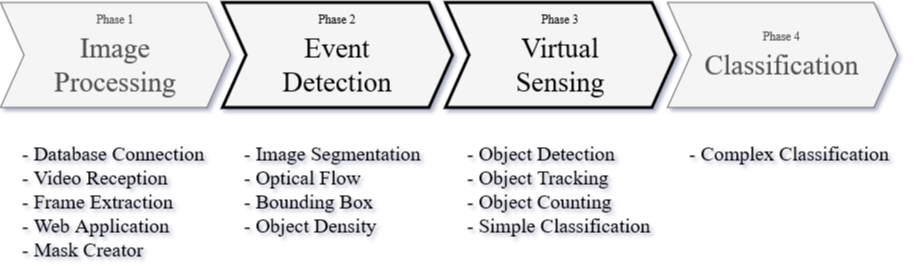
\includegraphics[width=0.95\textwidth]{proj_plan_02}
    \caption{Project Planning}
    \label{fig:proj_plan}
  \end{center}
\end{figure}


It is expected that this chapter provides some insight on how the theoretical backgrounds presented before were used during the project development, namely phase 2 and 3 of the planning presented in~\ref{fig:proj_plan}. Phase 2 focused on the detection of relevant events to the traffic controller such as suspicious approximation to the camera, intrusion in prohibited areas, fallen objects on the road and wrong way travelling, while phase 3 aimed to count and classify vehicles in both urban and high-way scenarios.

\section{Technology}

In order to build this project we needed both a library of already implemented computer vision algorithms as well as a simple way to retrieve frames from both video streams and files. This section describes what were the chosen technologies including a brief description and why it was chosen.

\subsection{OpenCV}
OpenCV is a library composed of implementations of useful computer vision algorithms implementation, widely used across the industry and academy. It has interfaces for multiple programming languages, like C++, Java and Python, but is natively written in C++ in order to take advantage of low level performance enhancements, as performance is an important factor in real time computer vision applications ~\cite{opencv_about_2017}.

The library contains over 2500 algorithms ranging from the more basic image processing, such as filtering, morphology operators and geometric transformations, to more complex ones that are able to compare images, track features, follow camera movements and recognize faces, among others. Along with the image processing capabilities, OpenCV also ships with interfaces to stereo cameras such as Kinect that allow users to retrieve a cloud of 3D points and a depth map from the captured image. This was the chosen library as there existed already previous work at LIACC using it, which could be leveraged for this project.

\subsection{JavaCV}
JavaCV is a wrapper for OpenCV written in Java that works on top of the JavaCPP Presets, a project that provides Java interfaces for commonly used C++ libraries, such as OpenCV and FFmpeg\todo{Adicionar referencias}, the ones we are using, as well as CUDA, ARToolKitPlus and others. It provides access to all the functionalities of OpenCV inside a Java environment, and was the chosen solution as there was already experience inside LIACC working with this technology.

Even though the code is written in Java and runs inside a Java Virtual Machine, the code from OpenCV is compiled from C/C++ and the memory of the objects created there is allocated in a separate thread. This made it impossible to rely on the garbage collector to do the memory management, and necessary to manually delete the native objects. Failure to address this issue causes the system to run out of memory and a subsequent program crash.

\subsection{FFmpeg}
FFmpeg is a framework that performs encoding, decoding, transcoding, streaming and filter operations in all the well known video formats, across a large number of platforms. It is used in the "Video Server" to read streams from any format and restream them all to the same format. In the Analytic module it is used to grab the frames from both the video files and the streams using the same code, as shown in ~\ref{src:ffmpegframegrabber}.

\begin{lstlisting}[float,language=Java, label={src:ffmpegframegrabber}, caption=FFmpegFrameGrabber usage example] 
// videopath can be either a stream path or a file path
FFmpegFrameGrabber _frameGrabber = FFmpegFrameGrabber.createDefault(videopath);
Frame currentFrame = null;

while( (currentFrame = _frameGrabber.grabImage()) != null) {
	// Use grabbed frame
}
\end{lstlisting}

\section{Architecture}

\subsection{Implementation Architecture}

\begin{figure}[h]
  \begin{center}
    \leavevmode
    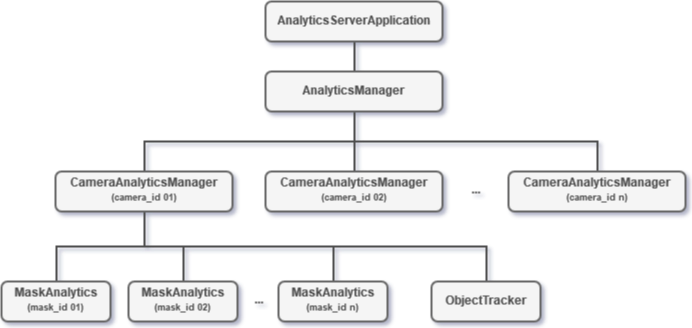
\includegraphics[width=0.95\textwidth]{ManagerArch}
    \caption{Manager Architecture}
    \label{fig:manager_arch}
  \end{center}
\end{figure}


The Analytics module was designed to comply with the following specifications, imposed by both our partner and to comply with the already developed modules. 

\begin{itemize}
	\item Run uninterruptedly waiting for requests to be made
	\item Process a large number of video inputs at the same time
	\item Receive input from streams or files
	\item Specify which analysis are to be run on a specific video
\end{itemize}
\todo{Mais requirements?}

The application main thread runs an instance of the AnalyticsManager class that implements the Java Runnable interface. This thread will launch one CameraAnalyticsManager instance for each video to be analysed, be it from stream or from file, and keep track of each worker status, disposing of them when they finish, and launching new ones when a request is received. The CameraAnalyticsManager is then responsible to query the database in order to find out what are the analytics the user wants to retrieve from the video through information that is stored in the \textit{camera} table of the database. This process then starts a frame grabber that will convert each frame of the video into its representation in OpenCV and feed it to each Analyser through a queue. This enables each one of these workers to run at his own pace and if one of them runs slower than the pace at which the frame grabber reads the images, it will simply queue them up and not slow down the remaining workers. The drawback of this solution is that it is theoretically possible to run out of memory to keep these frames, although this limit was not reached during the testing phase.

\section{Segmentation}

This section describes how the segmentation of the received images is performed, and how it returns a foreground mask representing the moving areas of the scene. 

\begin{figure}[h]
  \begin{center}
    \leavevmode
    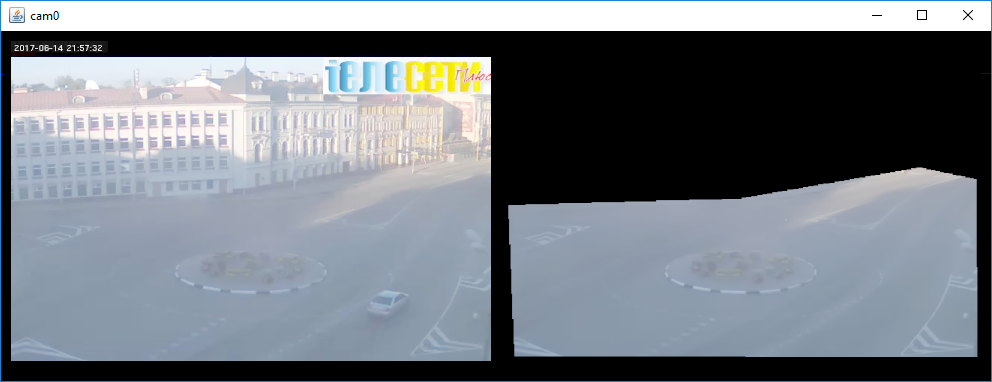
\includegraphics[width=0.95\textwidth]{bgsub_01}
    \caption{Background Subtraction - Background Model}
    \label{fig:bgsub_01}
  \end{center}
\end{figure}

In figure ~\ref{fig:bgsub_01} we can see the original frame on the left and the calculated background model of the scene on the right. To achieve this result, the first step is to mask the obtained frame \todo{Explain masking process} in order to prevent uninteresting regions of the image from being processed by the Background Subtracter. This solves an issue where moving or changing regions of the image outside our area of interest would create unwanted artefacts, for example moving trees due to the wind blowing, or the issue that occurred in this scene, where a car passing would be reflected in the windows of the building.

The next step of the Segmentation process is to feed the masked frames into a Background Subtraction algorithm that will use them to update its internal representation of the scene. This project uses the OpenCV implementation of the Mixture of Gaussians algorithm that allows the user to tune:

\begin{itemize}
	\item The number of past frames considered on the background calculation
	\item The threshold value from which a pixel is considered to be foreground, compared to the difference between its current value and the one from the background model
	\item The learning rate of the algorithm, how much each new frame influences the model
\end{itemize}

After updating the background model we can retrieve from the Background Subtracter its foreground mask, a rough representation that is calculated by subtracting the background model from the current image and thresholding it, thus returning only the pixels where the difference is significant enough.

\begin{figure}[h]
  \begin{center}
    \leavevmode
    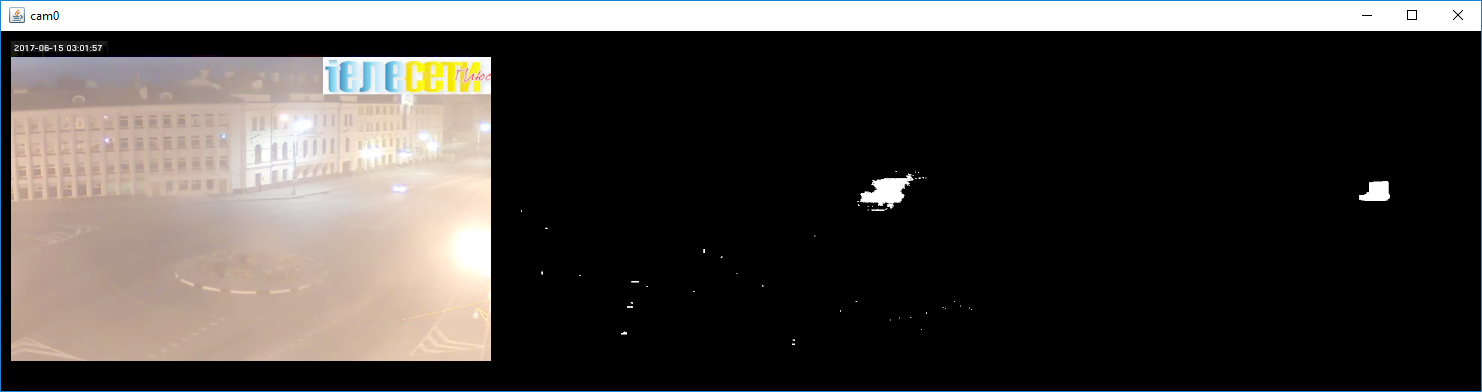
\includegraphics[width=0.95\textwidth]{bgsub_03}
    \caption{Background Subtraction - Foreground Mask}
    \label{fig:bgsub_02}
  \end{center}
\end{figure}

As we can see in the middle image of figure~\ref{fig:bgsub_02} the foreground mask from the Background Subtracter can have a lot of noise due to lighting conditions. To solve this issue two morphology filters are applied to the image: a squared erosion filter to remove the small speckles that appear in the mask; followed by a larger circular dilation filter to consolidate the positive regions of the mask, as the wind shield and windows of the vehicles are usually detected as background due to their dark colour and/or reflection of the environment.

\section{Object Detection}

This section describes how the information about the objects' size and position are retrieved from the binary mask returned from the segmentation process. 

OpenCV provides BlobDetector~\cite{opencv_opencv:_2017},  a family of functions that retrieve information of blobs in an image. It works by thresholding the input into multiple binary images using a range of threshold values, grouping the connected white pixels at each one of these images in binary blobs and then merging those that are close enough to each other into larger blobs. This method allows users to filter returned blobs based on 3 properties:

\begin{itemize}
	\item Area - The area of the region
	\item Circularity - Ratio between the area of the smallest involving circle and the area of the region
	\item Convexity - Ratio between the are of the convex hull of the region and its area
	\item Inertia - Elongation of the region (0 for lines, 1 for circles)
\end{itemize}

This however does not work as intended for our input, an already binarized image where we just need to group the connected pixels. For this the project uses the OpenCV function \textit{connectedComponentsWithStats}\todo{Italico para nomes de funçoes?}, that retrieves the groups of connected pixels in a binary image along with their area, width, height and both the leftmost and topmost coordinate of the group's bounding box. From this data we can create an ImageObject instance that will represent a moving object in the scene, using the regions with a size above a given threshold, in order to prevent detection of small objects or noise that got through the filtering process.

\section{Object Tracking}

In order for the solution to correctly analyse the objects of the scene it needs to track them during their lifetime, in other words, establish a relation between the objects identified on a frame with the objects identified in the next one. This is done by iterating through each one of the new objects and finding which existing object is closer to him. If the distance between them is smaller than the size of the existing object then they are matched.

\begin{figure}[h]
  \begin{center}
    \leavevmode
    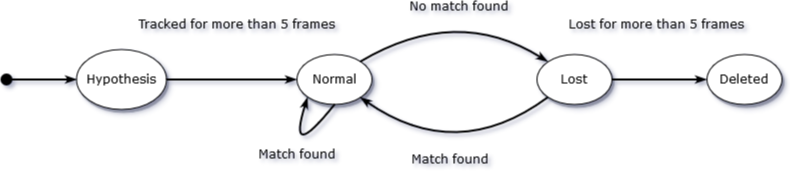
\includegraphics[width=0.95\textwidth]{state_machine_02}
    \caption{Object Life Cycle State Machine}
    \label{fig:object_state_machine}
  \end{center}
\end{figure}

To enhance this mechanism a sub-set of the state machine presented \todo{Referenciar artigo da state machine} which allows us to model the life cycle of an object. As seen in~\ref{fig:object_state_machine} an object starts as an Hypothesis, and cannot be used for analytics while in this state. After being tracked for 5 frames it then changes its state to Normal, where it stays until no match can be found, either from leaving the scene or due to problems with the input frame. An object in this state remains for a maximum of 5 frames, after which it is deleted or until a new object is found in the vicinities of it's last known position.

This technique relies on objects appearing close to their previous position in the next scene, and because the project was designed to run in high-way scenarios, where vehicles travel at high speeds, there was the need to improve it. The chosen solution was to follow a method used by Chris Dahms in his vehicle counting software ~\cite{dahms_opencv_3_car_counting_cpp_2017} that predicts an object next position by calculating an weighted average of the previous inter-position deltas and summing it to its current position as shown in ~\ref{eq:pos_pred}.

\begin{eqnarray}
\label{eq:pos_pred}
NextPos = CurrentPos + \sum_{i=1}^{5} (PosHist(i) - PosHist(i-1)) * (5-i)
\end{eqnarray}

In figure \ref{fig:object_tracking} we can see the result of the tracking process on the right most image. Each detected object is circled in a colour representing its current state in the state machine, blue for normal and red for lost, and shows the trail represents its path across the scene. 

\begin{figure}[h]
  \begin{center}
    \leavevmode
    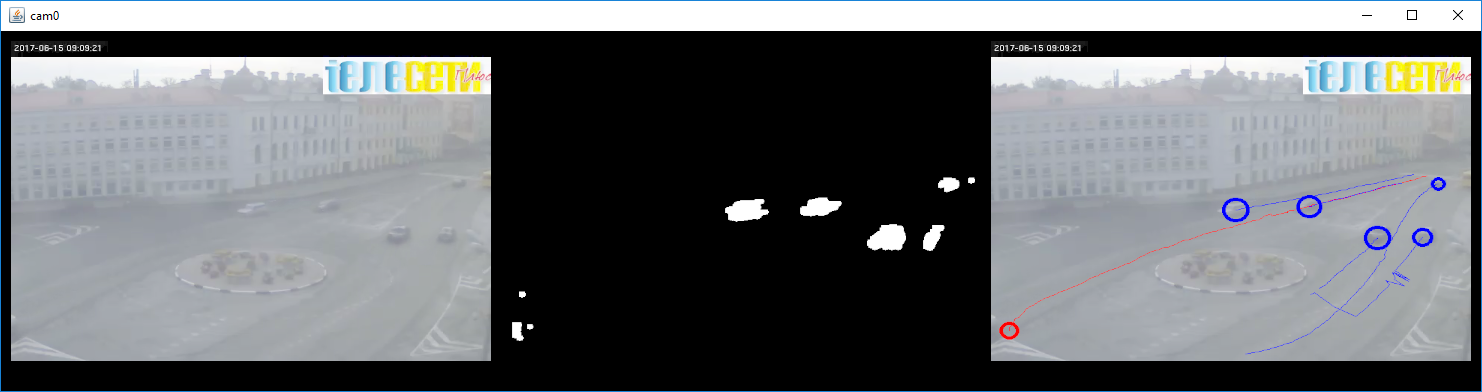
\includegraphics[width=0.95\textwidth]{object_01}
    \caption{Object Tracking}
    \label{fig:object_tracking}
  \end{center}
\end{figure}

\section{Object Classification}

\begin{figure}[h]
  \begin{center}
    \leavevmode
    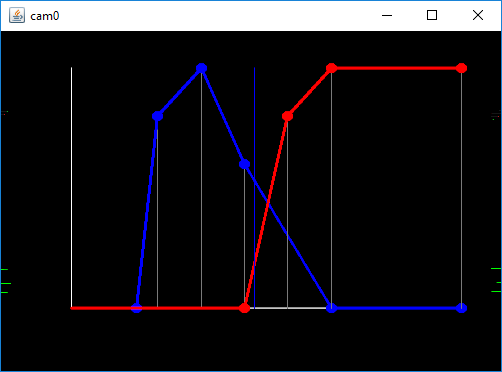
\includegraphics[width=0.5\textwidth]{classifier_01}
    \caption{Object Classifier}
    \label{fig:object_classifier}
  \end{center}
\end{figure}

In order to classify the objects present in the scene into light or heavy vehicles a fuzzy set is used. This set is calculated at run time based on a mask drawn by the user via the web interface that roughly approximates the size of a light vehicle. The area of that mask (A\textsubscript{Light}) is used as a base value to create the fuzzy set shown in figure \ref{fig:object_classifier}. This set has 2 series, one for light vehicles, drawn in blue, and one for heavy vehicles, drawn in red.

The blue series peaks at A\textsubscript{Light}, where we have 100\% certainty that a matched object is a light vehicle. The point immediate points are at 2/3*A\textsubscript{Light}, where the trust is 80\% and at 4/3*A\textsubscript{Light} where it drops to 60\%. Any object with area below 1/2*A\textsubscript{Light} or above 2*A\textsubscript{Light} are considered to have 0\% chance to be light vehicles.

The red series peaks at 2*A\textsubscript{Light}, and any object whose area is larger than this value is considered to be an heavy vehicle with 100\% confidence. At the same time, any object whose area is smaller than 4/3*A\textsubscript{Light} is never considered to be an heavy vehicle, from where the certainty rises to 80\% at 5/3*A\textsubscript{Light}.

When an object is counted in one of the virtual sensors its area is passed to this classifier where an interpolation is calculated for each series, returning the certainty with which it belongs to each one of the classes. Using these values the process can distinguish classifications with certainty below and above a user specified threshold to be treated separately.

\section{Feature Point Tracking}

\missingfigure{Feature Points}

The need to track feature points stems from the fact that without them we rely wholly on the background subtraction to process the image. Using feature points we can extract and track details of the vehicles that would otherwise be lost due to the process only working with a binary mask. 

We can use these points to distinguish vehicles grouped in a single binary region, as they are characterized by 
This way, even if a vehicle stops for a long time and starts to be considered background we can use its tracked points to maintain the position of \todo{Finish}

\section{Utility}

Over the development of the project the rise needed to implement some functionalities to enhance the code flow and to help the visualization of the implemented algorithms. This section will describe the most relevant ones for the reader to analyse and implement in its own projects.

\subsection{Video Wall}

\subsection{Image Processors}

\section{Summary}

Although dealing with a framework with no proper documentation was a difficult challenge to overcome, the performance obtained from the native code was essential for the final result, as the software is now able to track objects in a busy scene faster than the camera's capture rate, allowing us to process a video file in a shorter period of time than it's length. This was a request 